\documentclass{beamer}

\usepackage{hyperref}
\usepackage{amsmath}
\usepackage{amsfonts}
\usepackage[ruled]{algorithm}
\usepackage{algpseudocode}
\usepackage{graphicx}
\usepackage{minted}

\newcommand {\I} {\ensuremath {\mathbf{1\hspace{-5.5pt}1}}}
\renewcommand{\vec}[1]{\ensuremath{\boldsymbol{#1}}}

\title{Design and Implementation of\\Anglican Probabilistic Programming Language}
\author{David Tolpin \and Jan Willem van de Meent \and Hongseok Yang \and Frank Wood}
  
\AtBeginSection[]
{
  \begin{frame}<beamer>
    \frametitle{Outline}
    \tableofcontents[currentsection]
  \end{frame}
}

\begin{document}


\begin{frame}
\titlepage
\vfill
\center
\url{https://bitbucket.org/probprog/anglican-white-paper}\\
\url{https://bitbucket.org/probprog/anglican} \\
\url{http://www.robots.ox.ac.uk/~fwood/anglican/index.html}

\end{frame}

\section{Motivation}

\begin{frame}{Intuition}
    \textbf{Probabilistic program:}
\begin{itemize}
\item A program with random computations.
\item Distributions are conditioned by `observations'.
\item Values of certain expressions are `predicted' --- \textbf{the output}.
\end{itemize}

Can be written in any language (extended by \texttt{sample} and \texttt{observe}).
\end{frame}

\begin{frame}[fragile]{Example: Model Selection}
\begin{minted}[linenos, fontsize=\small]{clojure}
(let [;; Guessing a distribution
      dist (sample (categorical
                     [[normal 1] [gamma 1]
                      [uniform-continuous 1]
                      [uniform-discrete 1]]))
      a (sample (gamma 1 1))
      b (sample (gamma 1 1))
      d (dist a b)]

  ;; Observing samples from the distribution
  (loop [data data]
    (when (seq data)
      (let [[x & data] data]
        (observe d x))
      (recur data)))

  ;; Predicting a, b and the distribution
  (predict :a a) 
  (predict :b b)
  (predict :d d))
\end{minted}
\end{frame}

\begin{frame}{More examples}
    \begin{itemize}
        \item \textit{Intruder detection} --- 
            given a log of \textbf{times} and \textbf{amounts} of
            payments in a bank account, how likely that the baccount was
            compromised?
        \pause
        \item \textit{Counterfactual reasoning} --- There are
            \textbf{two routes} from Jerusalem to Tel Aviv:
            1 and 443.  Based on traffic reports, I chose route
            1 and was late. Would I arrive on time If I chose 443
            instead?
        \pause 
        \item \textit{(Due to Stuart Russell)} If you observe that a
            student GPA is exactly 4.0 in a model of
            transcripts of students from the USA (GPA's from
            0.0 to 4.0) and India (GPA's from 0.0 to
            10.0) what is the probability that the student
            is from India? 
    \end{itemize}
\end{frame}

\begin{frame}{Inference Objective}
\begin{itemize}
\item Suggest \textbf{most probable explanation} (MPE) - most likely assignment
  for all non-evidence variable given evidence.
  \pause
\item Approximately \textbf{compute integral} of the
  form $$\Phi=\int_{-\infty}^{\infty} \varphi(x)p(x) dx$$
  \pause
\item Continuously and \textbf{infinitely generate a sequence of samples} drawn
  from the distribution of the output expression --- so that someone
  else puts it in good use (vague but common). $\checkmark$
\end{itemize}
\end{frame}

\begin{frame}{Example: Inference Results}
  \begin{figure}[H]
      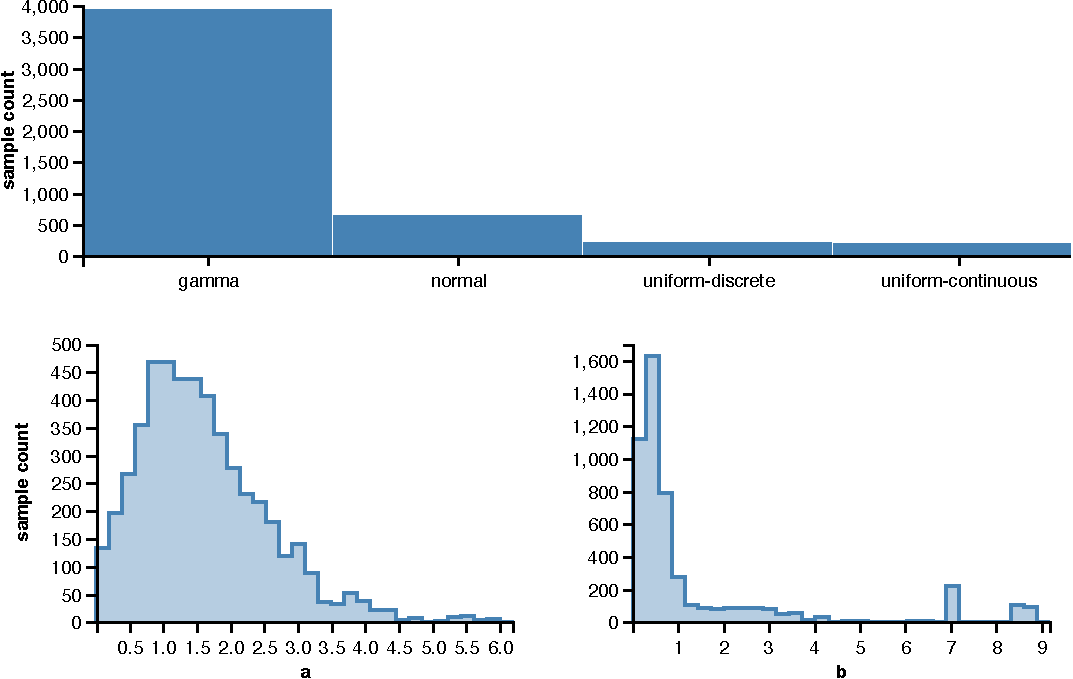
\includegraphics[scale=0.6]{models-results.pdf}
  \end{figure}
\end{frame}

\begin{frame}{Importance Sampling}
    \begin{algorithmic}
        \Loop
            \State Run program, computing weight based on observations.
            \State Output result and weight.
        \EndLoop
    \end{algorithmic}
    \begin{itemize}
        \item[] 
         \item Simple --- good.
         \item Slow convergence (unless one knows the answer) --- bad.
     \end{itemize}
     \vfill
     Can we do better?
\end{frame}

\begin{frame}{Lightweight Metropolis-Hastings (LMH)}
\begin{algorithmic}
    \State Run program once, remembering random choices.
    \Loop
         \State Uniformly select one random choice.
         \State Propose a new value for the choice.
         \State Re-run the program.
         \State Accept or reject with MH probability.
         \State Output result.
    \EndLoop
\end{algorithmic}
\vfill
Can we do better?
\begin{itemize}
    \item Particle methods
    \item Variational inference
    \item ...
\end{itemize}
\end{frame}

\begin{frame}{Why functional?}
    We want a functional language because an inference algorithm
    controls the execution:
    \begin{itemize}
        \item A program is run many (often many hundreds of
            thousands) of times (with almost any algorithm).
        \item A program must be partially re-executed multiple
            times from different positions (particle methods).
        \item We want to reason about the distribution defined
            by the program.
    \end{itemize}
\end{frame}

\begin{frame}{Why Closure?}
\begin{itemize}
    \item Runs on JVM --- easy deployment and access to libraries.
        \pause
    \item A Lisp --- we (ab)use the macro facility.
        \pause
    \item Church (\url{https://en.wikipedia.org/wiki/Church_(programming_language)}) is derived from Scheme.
\end{itemize}
\pause
Others use:
    \begin{itemize}
        \item Scheme --- (Church, Venture).
        \item Scala --- Figaro.
        \item Haskell --- Hakaru, Model-Bayes.
        \item ...
    \end{itemize}
    \pause
    As well as Python, C\#,  and other languages.
\end{frame}

\section{Design Outline}

\subsection{Language}

\subsection{Macro-based compilation}

\subsection{Implementation Highlights}

\subsection{Managing stack size}

\subsection{Probabilistic forms}

\subsection{Memoization}

\section{Inference Algorithms}

\section{Definitions and Runtime Library}

\begin{frame}
    \LARGE
    \center
    Thank you!\\Questions?
\end{frame}

\end{document}
